\documentclass[11pt, a4paper]{article}
\usepackage[utf8]{inputenc}
\usepackage[spanish]{babel}
\usepackage{amsmath, amssymb, amsfonts}
\usepackage{graphicx}
\usepackage{geometry}
\geometry{left=2.5cm, right=2.5cm, top=2.5cm, bottom=2.5cm}
\usepackage{tikz}
\usepackage{bm}
\usepackage[hidelinks]{hyperref}
\graphicspath{{figs/}{../figs/}}

% Línea discontinua entre ejercicios
\newcommand{\separador}{\par\vspace{0.3cm}\noindent\begin{tikzpicture}\draw[dashed] (0,0) -- (\linewidth,0);\end{tikzpicture}\par\vspace{0.3cm}}

\title{\vspace{-1.5cm}\textbf{Resolución de Ecuaciones Diferenciales Ordinarias}\\ \large Métodos Matemáticos I --- Hoja 5}
\author{\textbf{César Endris Acosta}}

\date{6 de noviembre de 2026}
\begin{document}

\maketitle
\vspace{-0.2cm}

\begin{center}
\fbox{\parbox{0.93\linewidth}{\small
\textbf{Versión interactiva.} Todos los problemas de esta hoja se pueden visualizar e interactuar con sus gráficas
(constantes con deslizadores, curva elegida, campos de direcciones, etc.) en la página web
(pestaña ``Hoja 5''):\\[2pt]
\centerline{\url{https://endris10.github.io/Mathematical_Methods_1/}}\vspace{2pt}
Se utilizó IA (Claude, de Anthropic) \textbf{únicamente para programar la página web};
la resolución de las ecuaciones diferenciales es propia.}}
\end{center}

\noindent\textbf{1. Verificad que la EDO $\bm{y''+y'-xy=0}$ tiene una fórmula de recurrencia de tres términos y hallad sus soluciones por series de potencias en $\bm{x}$: $\bm{y_1(x)}$ e $\bm{y_2(x)}$ tales que (a) $\bm{y_1(0)=1, y_1'(0)=0}$ (b) $\bm{y_2(0)=0, y_2'(0)=1}$} \\

Proponemos $y(x) = \sum_{n=0}^{\infty} a_n x^n$. Derivando:
\begin{align*}
y' = \sum_{n=0}^{\infty} (n+1)a_{n+1} x^n, \qquad y'' = \sum_{n=0}^{\infty} (n+2)(n+1)a_{n+2} x^n
\end{align*}
Sustituimos en la EDO:
\begin{align*}
\sum_{n=0}^{\infty} (n+2)(n+1)a_{n+2} x^n + \sum_{n=0}^{\infty} (n+1)a_{n+1} x^n - \sum_{n=0}^{\infty} a_n x^{n+1} = 0
\end{align*}
Corremos el índice en el último sumatorio ($n \to n-1$), asumiendo que los coeficientes con subíndices negativos son cero ($a_{-1} = 0$):
\begin{align*}
\sum_{n=0}^{\infty} \left[ (n+2)(n+1)a_{n+2} + (n+1)a_{n+1} - a_{n-1} \right] x^n = 0
\end{align*}
Igualando a cero el coeficiente general para todo $n \geq 0$, obtenemos la \textbf{fórmula de recurrencia de tres términos}:
\begin{align*}
a_{n+2} = \frac{a_{n-1} - (n+1)a_{n+1}}{(n+2)(n+1)}
\end{align*}
Evaluamos:
\begin{align*}
n=0 &\implies a_2 = \frac{a_{-1} - a_1}{2} = -\frac{a_1}{2} \\
n=1 &\implies a_3 = \frac{a_0 - 2a_2}{6} = \frac{a_0 - 2(-a_1/2)}{6} = \frac{a_0}{6} + \frac{a_1}{6} \\
n=2 &\implies a_4 = \frac{a_1 - 3a_3}{12} = \frac{a_1 - 3(a_0/6 + a_1/6)}{12} = \frac{a_1 - a_0/2 - a_1/2}{12} = -\frac{a_0}{24} + \frac{a_1}{24} \\
n=3 &\implies a_5 = \frac{a_2 - 4a_4}{20} = \frac{-a_1/2 - 4(-a_0/24 + a_1/24)}{20} = \frac{a_0}{120} - \frac{a_1}{30}
\end{align*}

\begin{align*}
y(x) &= a_0 + a_1 x + a_2 x^2 + a_3 x^3 + a_4 x^4 + a_5 x^5 + \dots \\
&= a_0\left(1 + \frac{1}{6}x^3 - \frac{1}{24}x^4 + \frac{1}{120}x^5 + \dots\right) + a_1\left(x - \frac{1}{2}x^2 + \frac{1}{6}x^3 + \frac{1}{24}x^4 - \frac{1}{30}x^5 + \dots\right)
\end{align*}

Ahora para las condiciones iniciales:
\begin{itemize}
\item \textbf{(a) $\bm{y_1(0)=1}$ e $\bm{y_1'(0)=0}$}: \\
Evaluando en la solución general, tenemos que $y(0) = a_0 = 1$ y $y'(0) = a_1 = 0$. Por lo tanto, la primera solución particular es la serie multiplicada por $a_0$:
\[
\boxed{y_1(x) = 1 + \frac{1}{6}x^3 - \frac{1}{24}x^4 + \frac{1}{120}x^5 + \dots}
\]


\begin{center}
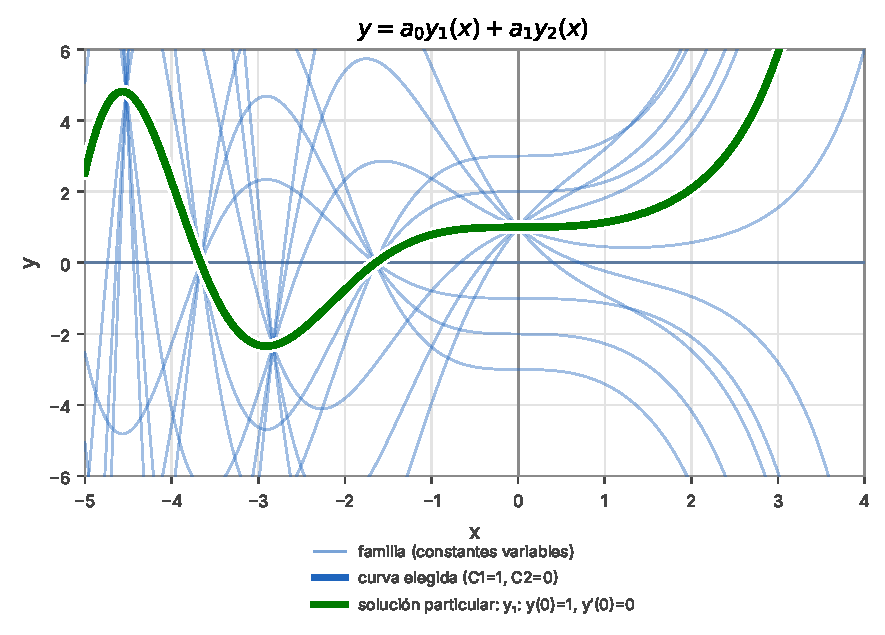
\includegraphics[width=0.8\linewidth]{h5-01-a.pdf}
\end{center}
\item \textbf{(b) $\bm{y_2(0)=0}$ e $\bm{y_2'(0)=1}$}: \\
Evaluando, tenemos que $y(0) = a_0 = 0$ y $y'(0) = a_1 = 1$. Por lo tanto, la segunda solución particular es solo la serie multiplicada por $a_1$:
\[
\boxed{y_2(x) = x - \frac{1}{2}x^2 + \frac{1}{6}x^3 + \frac{1}{24}x^4 - \frac{1}{30}x^5 + \dots}
\]

\begin{center}
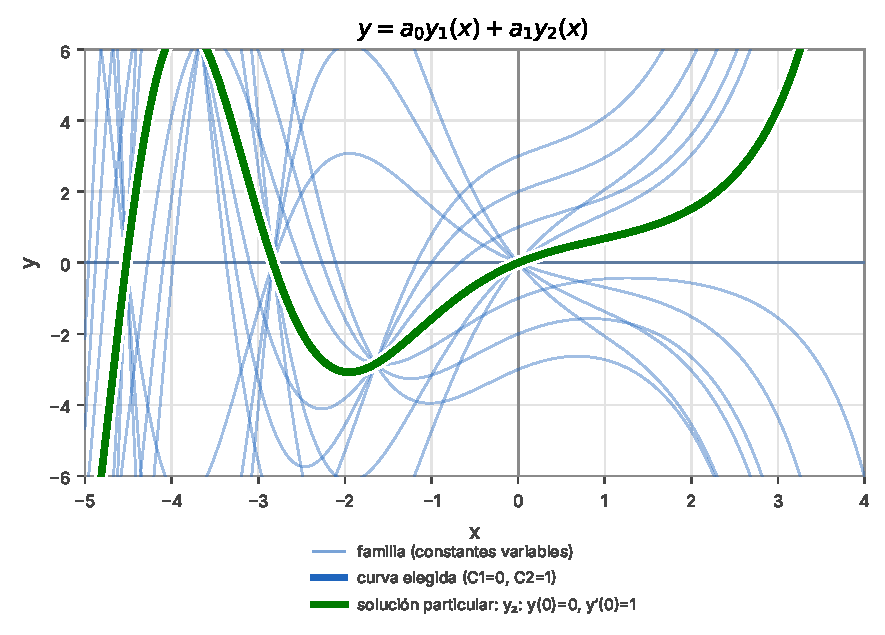
\includegraphics[width=0.8\linewidth]{h5-01-b.pdf}
\end{center}
\end{itemize}


\noindent\textbf{2. La EDO $\bm{y''+(p+\frac{1}{2}-\frac{x^2}{4})y=0}$, donde $\bm{p}$ es una constante, tiene una solución en serie de la forma $\bm{y=\sum a_{n}x^{n}}$: (a) demostrad que los coeficientes $\bm{a_{n}}$ están relacionados por una fórmula de recurrencia de tres términos; (b) si se hace el cambio de variable dependiente $\bm{y=we^{-x^2/4}}$, probad que la EDO original se transforma en $\bm{w''-xw'+pw=0}$; (c) comprobad que la EDO para $\bm{w}$ tiene una fórmula de recurrencia de dos términos y hallad la solución general.} \\
\textbf{(a) Demostrad que hay una recurrencia de 3 términos para $\bm{y=\sum a_n x^n}$:} \\
Proponemos $y = \sum_{n=0}^{\infty} a_n x^n$. Derivando dos veces:
\begin{align*}
y'' = \sum_{n=0}^{\infty} (n+2)(n+1)a_{n+2} x^n
\end{align*}
Sustituyendo en la EDO:
\begin{align*}
\sum_{n=0}^{\infty} (n+2)(n+1)a_{n+2} x^n + \left(p+\frac{1}{2}\right)\sum_{n=0}^{\infty} a_n x^n - \frac{1}{4}\sum_{n=0}^{\infty} a_n x^{n+2} &= 0
\end{align*}
Agrupamos todo bajo la misma potencia, $x^n$, ajustando ($n \to n-2$) en el último término. Asumiendo por definición que $a_{-2} = 0$ y $a_{-1} = 0$:
\begin{align*}
\sum_{n=0}^{\infty} \left[ (n+2)(n+1)a_{n+2} + \left(p+\frac{1}{2}\right)a_n - \frac{1}{4}a_{n-2} \right] x^n &= 0
\end{align*}
Igualando a cero el coeficiente general para todo $n \geq 0$, obtenemos la \textbf{fórmula de recurrencia de tres términos}:
\begin{align*}
a_{n+2} = \frac{\frac{1}{4}a_{n-2} - \left(p+\frac{1}{2}\right)a_n}{(n+2)(n+1)}
\end{align*}
Vemos claramente que cada coeficiente $a_{n+2}$ depende de los dos anteriores con la misma paridad ($a_n$ y $a_{n-2}$), conformando así una recurrencia de tres términos. \quad $\blacksquare$

\vspace{0.2cm}\noindent\textbf{(b) Cambio $\bm{y=we^{-x^2/4}}$:} \\
\begin{align*}
y' &= \left(w' - \frac{x}{2}w\right)e^{-x^2/4} \\
y'' &= \left[w'' - \frac{1}{2}w - \frac{x}{2}w' - \frac{x}{2}\left(w' - \frac{x}{2}w\right)\right]e^{-x^2/4} = \left(w'' - xw' + \frac{x^2}{4}w - \frac{1}{2}w\right)e^{-x^2/4}
\end{align*}
Dividiendo entre $e^{-x^2/4}$:
\begin{align*}
\left(w'' - xw' + \frac{x^2}{4}w - \frac{1}{2}w\right) + \left(p + \frac{1}{2} - \frac{x^2}{4}\right)w &= 0 \implies w'' - xw' + pw = 0 \quad \blacksquare
\end{align*}

\vspace{0.2cm}\noindent\textbf{(c) EDO para $\bm{w}$ y solución general:} \\
Sustituimos $w = \sum a_n x^n$ en $w'' - xw' + pw = 0$:
\begin{align*}
\sum_{n=0}^{\infty} (n+2)(n+1)a_{n+2} x^n - \sum_{n=0}^{\infty} n a_n x^n + \sum_{n=0}^{\infty} p a_n x^n &= 0 \\
\sum_{n=0}^{\infty} \big[ (n+2)(n+1)a_{n+2} - (n-p)a_n \big] x^n &= 0
\end{align*}
Fórmula de recurrencia (2 términos): $a_{n+2} = \dfrac{n-p}{(n+2)(n+1)} a_n$.
\begin{align*}
n=0 &\implies a_2 = \frac{-p}{2}a_0 \\
n=2 &\implies a_4 = \frac{2-p}{12}a_2 = \frac{-p(2-p)}{24}a_0 \\
n=1 &\implies a_3 = \frac{1-p}{6}a_1 \\
n=3 &\implies a_5 = \frac{3-p}{20}a_3 = \frac{(1-p)(3-p)}{120}a_1
\end{align*}
La solución general es $y(x) = w(x)e^{-x^2/4}$:
\[
\boxed{y(x) = e^{-x^2/4} \left[ a_0\left(1 - \frac{p}{2}x^2 - \frac{p(2-p)}{24}x^4 + \dots\right) + a_1\left(x + \frac{1-p}{6}x^3 + \frac{(1-p)(3-p)}{120}x^5 + \dots\right) \right]}
\]



\begin{center}
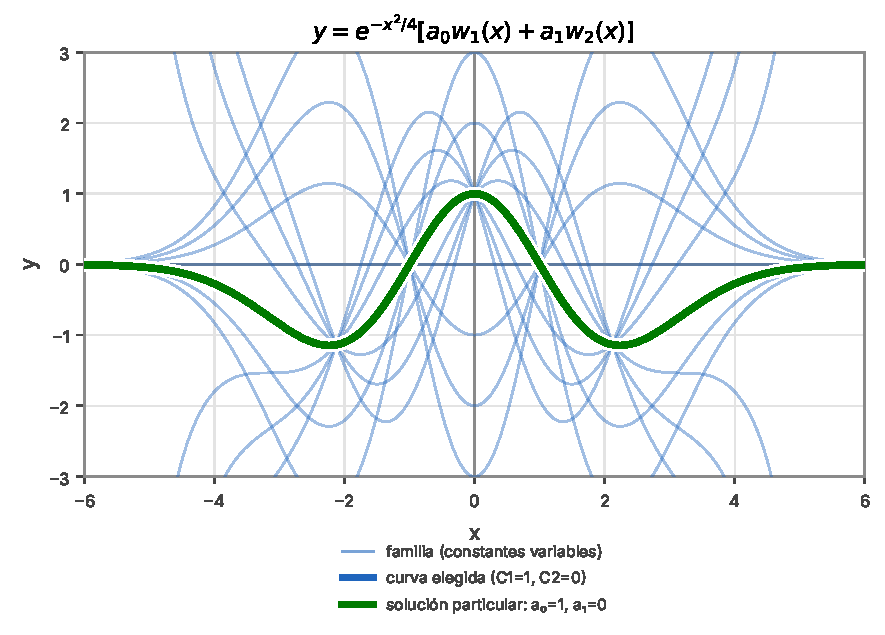
\includegraphics[width=0.8\linewidth]{h5-02.pdf}
\end{center}

\noindent\textbf{3. Las soluciones de la ecuación de Airy $\bm{y''+xy=0}$ se llaman funciones de Airy. Hallad las funciones de Airy en forma de serie de potencias en $\bm{x}$ y comprobad directamente que las series obtenidas convergen para todo $\bm{x}$. Usando dichos resultados, obtened la solución general de la EDO $\bm{y''-xy=0}$ sin hacer cálculos.} \\
Sustituyendo en $y''+xy=0$:
\begin{align*}
\sum_{n=0}^{\infty} (n+2)(n+1)a_{n+2} x^n + \sum_{n=0}^{\infty} a_n x^{n+1} &= 0
\end{align*}
\begin{align*}
\sum_{n=0}^{\infty} \big[ (n+2)(n+1)a_{n+2} + a_{n-1} \big] x^n &= 0
\end{align*}
\begin{align*}
a_{n+2} = \frac{-a_{n-1}}{(n+2)(n+1)}
\end{align*}
Evaluamos los primeros términos:
\begin{align*}
n=0 &\implies a_2 = \frac{-a_{-1}}{2\cdot 1} = 0 \\
n=1 &\implies a_3 = \frac{-a_0}{3\cdot 2} = -\frac{a_0}{6} \\
n=2 &\implies a_4 = \frac{-a_1}{4\cdot 3} = -\frac{a_1}{12} \\
n=3 &\implies a_5 = \frac{-a_2}{5\cdot 4} = 0 \\
n=4 &\implies a_6 = \frac{-a_3}{6\cdot 5} = \frac{-(-a_0/6)}{30} = \frac{a_0}{180} \\
n=5 &\implies a_7 = \frac{-a_4}{7\cdot 6} = \frac{-(-a_1/12)}{42} = \frac{a_1}{504}
\end{align*}
Los coeficientes dan saltos de 3 en 3 (siendo siempre nulos los de la forma $a_{3k+2}$). La fórmula general luego es:
\begin{align*}
a_{3k} &= a_0 \frac{(-1)^k}{2\cdot 3 \cdot 5\cdot 6 \cdots (3k-1)(3k)}, \qquad a_{3k+1} = a_1 \frac{(-1)^k}{3\cdot 4 \cdot 6\cdot 7 \cdots (3k)(3k+1)}
\end{align*}

Agrupando, las funciones de Airy en serie (la solución homogénea general) son:
\begin{align*}
y(x) = a_0\underbrace{\left(1 - \frac{1}{6}x^3 + \frac{1}{180}x^6 - \dots\right)}_{y_1(x)} + a_1\underbrace{\left(x - \frac{1}{12}x^4 + \frac{1}{504}x^7 - \dots\right)}_{y_2(x)}
\end{align*}
Convergencia (Aplicamos la Prueba del Cociente): 
\begin{align*}
L = \lim_{k\to\infty} \left| \frac{a_{3(k+1)}x^{3(k+1)}}{a_{3k}x^{3k}} \right| = \lim_{k\to\infty} \left| \frac{-x^3}{(3k+2)(3k+3)} \right| = 0 < 1 \implies R = \infty \quad \forall x \in \mathbb{R} \quad \blacksquare
\end{align*}
Para resolver la segunda EDO $y''-xy=0$, hacemos el cambio $x \to -x$. Entonces, la solución para la nueva EDO se obtiene evaluando las series encontradas en $-x$:
\[
\boxed{y(x) = a_0\left(1 + \frac{1}{6}x^3 + \frac{1}{180}x^6 + \dots\right) + a_1\left(x + \frac{1}{12}x^4 + \frac{1}{504}x^7 + \dots\right)}
\]



\begin{center}
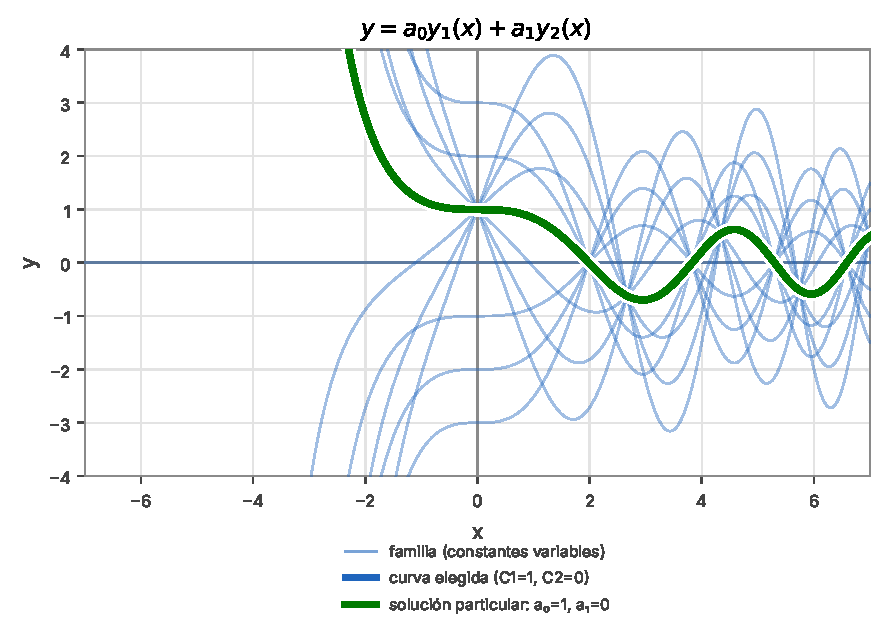
\includegraphics[width=0.8\linewidth]{h5-03.pdf}
\end{center}

\noindent\textbf{4. La ecuación de Chebyshev es $\bm{(1-x^2)y''-xy'+p^2y=0}$ donde $\bm{p}$ es una constante. Hallad dos soluciones en serie de potencias linealmente independientes que sean soluciones válidas en $\bm{|x|<1}$. Probad que si $\bm{p=n}$, donde $\bm{n}$ es un entero positivo, existe un polinomio de grado $\bm{n}$ que es solución (cuando éstos se multiplican por constantes adecuadas se denominan polinomios de Chebyshev).} \\
Proponemos $y = \sum a_n x^n$:
\begin{align*}
\sum_{n=0}^{\infty} (n+2)(n+1)a_{n+2} x^n - \sum_{n=0}^{\infty} n(n-1)a_n x^n - \sum_{n=0}^{\infty} n a_n x^n + \sum_{n=0}^{\infty} p^2 a_n x^n &= 0 \\
\sum_{n=0}^{\infty} \big[ (n+2)(n+1)a_{n+2} - (n^2 - p^2)a_n \big] x^n &= 0
\end{align*}
Fórmula de recurrencia: $a_{n+2} = \frac{n^2-p^2}{(n+2)(n+1)} a_n$.\\
\begin{itemize}
\item \textbf{Rama par:}
\begin{align*}
n=0 &\implies a_2 = \frac{0^2 - p^2}{2\cdot 1} a_0 = -\frac{p^2}{2!} a_0 \\
n=2 &\implies a_4 = \frac{2^2 - p^2}{4\cdot 3} a_2 = \frac{(4 - p^2)(-p^2)}{4!} a_0
\end{align*}
\item \textbf{Rama impar:}
\begin{align*}
n=1 &\implies a_3 = \frac{1^2 - p^2}{3\cdot 2} a_1 = \frac{1 - p^2}{3!} a_1 \\
n=3 &\implies a_5 = \frac{3^2 - p^2}{5\cdot 4} a_3 = \frac{(9 - p^2)(1 - p^2)}{5!} a_1
\end{align*}
\end{itemize}

Resolviendo para las ramas par e impar:
\begin{align*}
y_1(x) &= 1 - \frac{p^2}{2!}x^2 + \frac{(2^2-p^2)(-p^2)}{4!}x^4 + \dots \\
y_2(x) &= x + \frac{1-p^2}{3!}x^3 + \frac{(3^2-p^2)(1-p^2)}{5!}x^5 + \dots
\end{align*}
Prueba del cociente: $L = \lim_{n\to\infty} \left| \frac{n^2-p^2}{(n+2)(n+1)} x^2 \right| = |x^2|$. Converge si $|x| < 1$. \\
Si $p=n$ (donde $n$ es un entero positivo), en la fórmula de recurrencia $a_{k+2} = \frac{k^2 - n^2}{(k+2)(k+1)} a_k$ al evaluar en el índice $k = n$, el numerador se anula:
\begin{align*}
a_{n+2} = \frac{n^2 - n^2}{(n+2)(n+1)} a_n = 0
\end{align*}
Por lo tanto, a partir de ese término, $a_{n+2} = 0$ y, de forma sucesiva, todos los coeficientes siguientes con la misma paridad también se anulan ($a_{n+4} = 0, a_{n+6} = 0, \dots$). Esto hace que la serie infinita se convierta en un polinomio exacto de grado $n$, siendo por tanto una solución válida. \quad $\blacksquare$ \\


\begin{center}
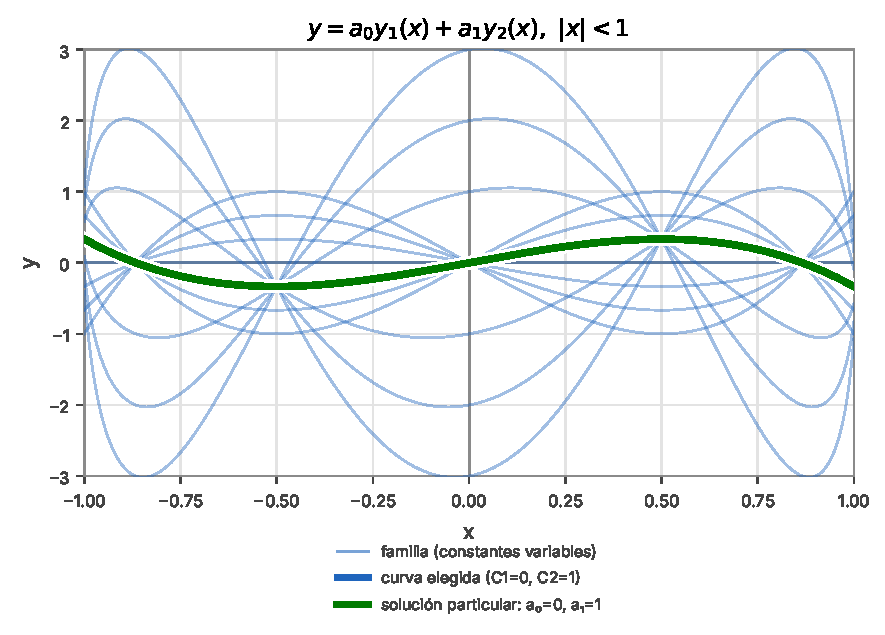
\includegraphics[width=0.8\linewidth]{h5-04.pdf}
\end{center}

\noindent {\bfseries 5. La ecuación de Hermite es $\bm{y''-2xy'+2py=0}$ donde $\bm{p}$ es una constante:\\ 
(a) Demostrad que su solución general es $\bm{y(x)=a_0 y_1(x)+a_1 y_2(x)}$, donde\\ 
$\boldsymbol{y_1(x)=1-\frac{2p}{2!}x^2+\frac{2^2 p(p-2)}{4!}x^4-\frac{2^3 p(p-2)(p-4)}{6!}x^6+\cdots}$ y\\ 
$\boldsymbol{y_2(x)=x-\frac{2(p-1)}{3!}x^3+\frac{2^2 (p-1)(p-3)}{5!}x^5-\frac{2^3 (p-1)(p-3)(p-5)}{7!}x^7+\cdots}$.\\ 
Por el teorema mencionado en clase ambas series convergen para todo $\bm{x}$. Comprobadlo directamente.\\ 
(b) Si $\bm{p}$ es un entero no negativo, una de esas series termina y se reduce a un polinomio, mientras que la otra sigue siendo una serie infinita. Verificad que para $\bm{p=0,1,2,3,4,5}$, esos polinomios son $\bm{1}$, $\bm{x}$, $\bm{1-2x^2}$, $\bm{x-2x^3/3}$, $\bm{1-4x^2+4x^4/3}$ y $\bm{x-4x^3/3+4x^5/15}$.\\ 
(c) Es claro que las únicas soluciones polinómicas de la ecuación de Hermite son múltiplos constantes de los polinomios descritos en (b). Aquellos múltiplos constantes cuyos términos dominantes son de la forma $\bm{2^n x^n}$ se denotan por $\bm{H_n(x)}$ y se denominan polinomios de Hermite. Hallad $\bm{H_n(x)}$ para $\bm{n=0,1,2,3,4,5}$.\\ 
(d) Verificad que los polinomios hallados en (c) vienen dados por la fórmula general $\bm{H_n(x)=(-1)^n e^{x^2}\frac{d^n}{dx^n}e^{-x^2}}$.} \\

\textbf{(a) General y convergencia:}
\begin{align*}
\sum_{n=0}^{\infty} (n+2)(n+1)a_{n+2} x^n - \sum_{n=0}^{\infty} 2n a_n x^n + \sum_{n=0}^{\infty} 2p a_n x^n &= 0 \implies a_{n+2} = \frac{2(n-p)}{(n+2)(n+1)} a_n
\end{align*}
Evaluando $a_2, a_3, a_4\dots$ se recuperan exactamente las series $y_1(x)$ y $y_2(x)$ dadas en el enunciado. \\
Convergencia: $L = \lim_{n\to\infty} \left| \frac{2(n-p)}{(n+2)(n+1)} x^2 \right| = 0 \implies$ Converge para todo $x \in \mathbb{R}$. \quad $\blacksquare$

\vspace{0.2cm}\noindent\textbf{(b) Polinomios no normalizados para $\bm{p=0,1,2,3,4,5}$:}
\begin{itemize}
\item $p=0 \implies y_1 = 1$.
\item $p=1 \implies y_2 = x$.
\item $p=2 \implies y_1 = 1 - \frac{4}{2}x^2 = 1 - 2x^2$.
\item $p=3 \implies y_2 = x - \frac{4}{6}x^3 = x - \frac{2}{3}x^3$.
\item $p=4 \implies y_1 = 1 - \frac{8}{2}x^2 + \frac{16(2)}{24}x^4 = 1 - 4x^2 + \frac{4}{3}x^4$.
\item $p=5 \implies y_2 = x - \frac{8}{6}x^3 + \frac{16(2)}{120}x^5 = x - \frac{4}{3}x^3 + \frac{4}{15}x^5$. \quad $\checkmark$
\end{itemize}

\vspace{0.2cm}\noindent\textbf{(c) Polinomios de Hermite $\bm{H_n(x)}$ (con término dominante $\bm{2^n x^n}$):}
\begin{itemize}
\item $H_0(x) = 1 \cdot (1) = \mathbf{1}$
\item $H_1(x) = 2 \cdot (x) = \mathbf{2x}$
\item $H_2(x) = (-2) \cdot (1 - 2x^2) = \mathbf{4x^2 - 2}$
\item $H_3(x) = (-12) \cdot \left(x - \frac{2}{3}x^3\right) = \mathbf{8x^3 - 12x}$
\item $H_4(x) = (12) \cdot \left(1 - 4x^2 + \frac{4}{3}x^4\right) = \mathbf{16x^4 - 48x^2 + 12}$
\item $H_5(x) = (120) \cdot \left(x - \frac{4}{3}x^3 + \frac{4}{15}x^5\right) = \mathbf{32x^5 - 160x^3 + 120x}$
\end{itemize}

\vspace{0.2cm}\noindent\textbf{(d) $\bm{H_n(x) = (-1)^n e^{x^2} \frac{d^n}{dx^n} e^{-x^2}}$ :} \\
 Evaluando:
\begin{align*}
n=0 &\implies e^{x^2} e^{-x^2} = 1 = H_0 \\
n=1 &\implies -e^{x^2} (-2x e^{-x^2}) = 2x = H_1 \\
n=2 &\implies e^{x^2} \frac{d}{dx}(-2x e^{-x^2}) = e^{x^2}(-2 + 4x^2)e^{-x^2} = 4x^2 - 2 = H_2
\end{align*}
Los polinomios coinciden. \quad $\blacksquare$



\begin{center}
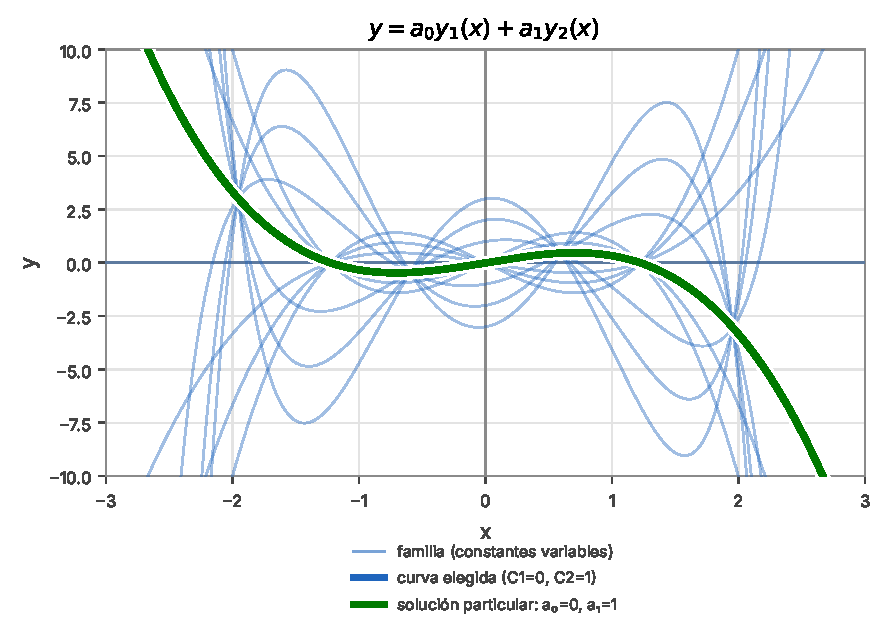
\includegraphics[width=0.8\linewidth]{h5-05.pdf}
\end{center}

\noindent\textbf{6. Sea la EDO $\bm{y''-xy'-2y=0}$. Hallad dos soluciones en serie de potencias en $\bm{x}$ linealmente independientes, estudiad sus radios de convergencia y escribid la solución general.} \\
\begin{align*}
\sum_{n=0}^{\infty} (n+2)(n+1)a_{n+2} x^n - \sum_{n=0}^{\infty} n a_n x^n - \sum_{n=0}^{\infty} 2 a_n x^n &= 0 \\
\sum_{n=0}^{\infty} \big[ (n+2)(n+1)a_{n+2} - (n+2)a_n \big] x^n &= 0 \implies a_{n+2} = \frac{1}{n+1} a_n
\end{align*}
Calculando para índices pares e impares:
\begin{align*}
a_2 &= a_0, \quad a_4 = \frac{1}{3}a_2 = \frac{1}{3}a_0, \quad a_6 = \frac{1}{5}a_4 = \frac{1}{15}a_0 \implies y_1(x) = 1 + x^2 + \frac{x^4}{3} + \frac{x^6}{15} + \dots \\
a_3 &= \frac{1}{2}a_1, \quad a_5 = \frac{1}{4}a_3 = \frac{1}{8}a_1, \quad a_7 = \frac{1}{6}a_5 = \frac{1}{48}a_1 \implies y_2(x) = x + \frac{x^3}{2} + \frac{x^5}{8} + \frac{x^7}{48} + \dots 
\end{align*}
Prueba del cociente: $L = \lim_{n\to\infty} \left| \frac{1}{n+1} x^2 \right| = 0 < 1 \implies R = \infty$. 
\[
\boxed{y(x) = a_0\left(1 + x^2 + \frac{x^4}{3} + \frac{x^6}{15} + \dots\right) + a_1\left(x + \frac{x^3}{2} + \frac{x^5}{8} + \frac{x^7}{48} + \dots\right)}
\]


\begin{center}
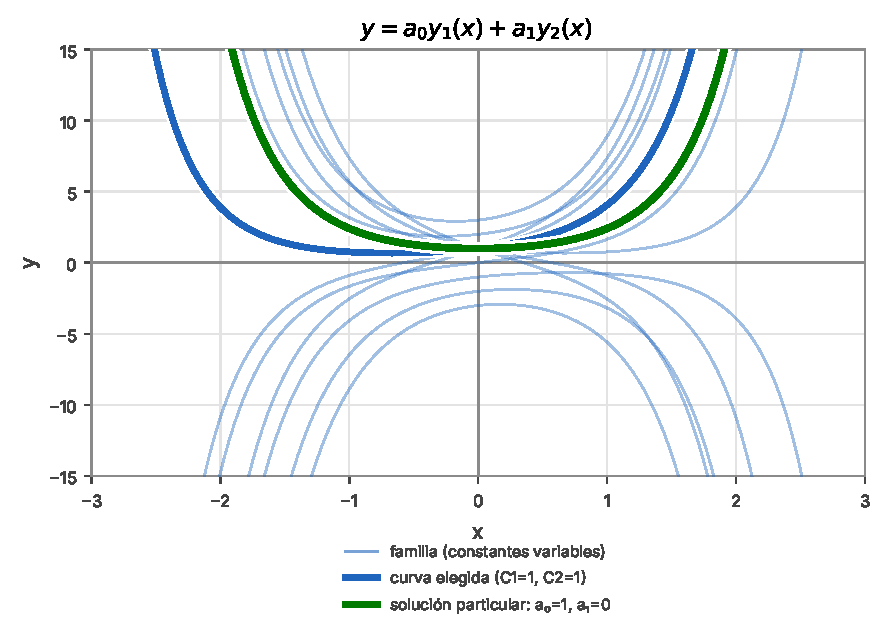
\includegraphics[width=0.8\linewidth]{h5-06.pdf}
\end{center}

\noindent\textbf{7. Sea la EDO $\bm{y''+x^2 y=1+x+x^2}$. Hallad la solución general en términos de series de potencias en $\bm{x}$.} \\
\begin{align*}
\sum_{n=0}^{\infty} (n+2)(n+1)a_{n+2} x^n + \sum_{n=0}^{\infty} a_n x^{n+2} &= 1 + x + x^2 \\
\end{align*}
El términode la derecha se puede expresarse como otra serie finita $f(x) = 1 + x + x^2 = \sum_{n=0}^{\infty} b_n x^n$, cuyos coeficientes son:
\begin{align*}
b_0 = 1, \quad b_1 = 1, \quad b_2 = 1, \quad \text{y} \quad b_n = 0 \quad \text{para } n \geq 3
\end{align*}
Sustituyendo:
\begin{align*}
\sum_{n=0}^{\infty} (n+2)(n+1)a_{n+2} x^n + \sum_{n=0}^{\infty} a_n x^{n+2} &= \sum_{n=0}^{\infty} b_n x^n \\
\sum_{n=0}^{\infty} (n+2)(n+1)a_{n+2} x^n + \sum_{n=2}^{\infty} a_{n-2} x^n &= \sum_{n=0}^{\infty} b_n x^n \\
\sum_{n=0}^{\infty} \big[ (n+2)(n+1)a_{n+2} + a_{n-2} - b_n \big] x^n = 0
\end{align*}
Conseguimos la relación de recurrencia general:
\begin{align*}
a_{n+2} = \frac{b_n - a_{n-2}}{(n+2)(n+1)}
\end{align*}
Evaluamos:
\begin{align*}
n=0: &\quad a_2 = \frac{b_0 - a_{-2}}{2\cdot 1} = \frac{1 - 0}{2} = \frac{1}{2} \\
n=1: &\quad a_3 = \frac{b_1 - a_{-1}}{3\cdot 2} = \frac{1 - 0}{6} = \frac{1}{6} \\
n=2: &\quad a_4 = \frac{b_2 - a_0}{4\cdot 3} = \frac{1 - a_0}{12} \\
n=3: &\quad a_5 = \frac{b_3 - a_1}{5\cdot 4} = \frac{0 - a_1}{20} = -\frac{a_1}{20} \\
n=4: &\quad a_6 = \frac{b_4 - a_2}{6\cdot 5} = \frac{0 - (1/2)}{30} = -\frac{1}{60} \\
n=5: &\quad a_7 = \frac{b_5 - a_3}{7\cdot 6} = \frac{0 - (1/6)}{42} = -\frac{1}{252}
\end{align*}
Agrupando la solución general en su parte homogénea $y_h$ (dependiente de $a_0$ y $a_1$) y su parte particular $y_p$:
\[
\boxed{y(x) = a_0\left(1 - \frac{x^4}{12} + \frac{x^8}{672} - \dots\right) + a_1\left(x - \frac{x^5}{20} + \dots\right) + \left(\frac{x^2}{2} + \frac{x^3}{6} + \frac{x^4}{12} - \frac{x^6}{60} - \frac{x^7}{252} \dots\right)}
\]


\begin{center}
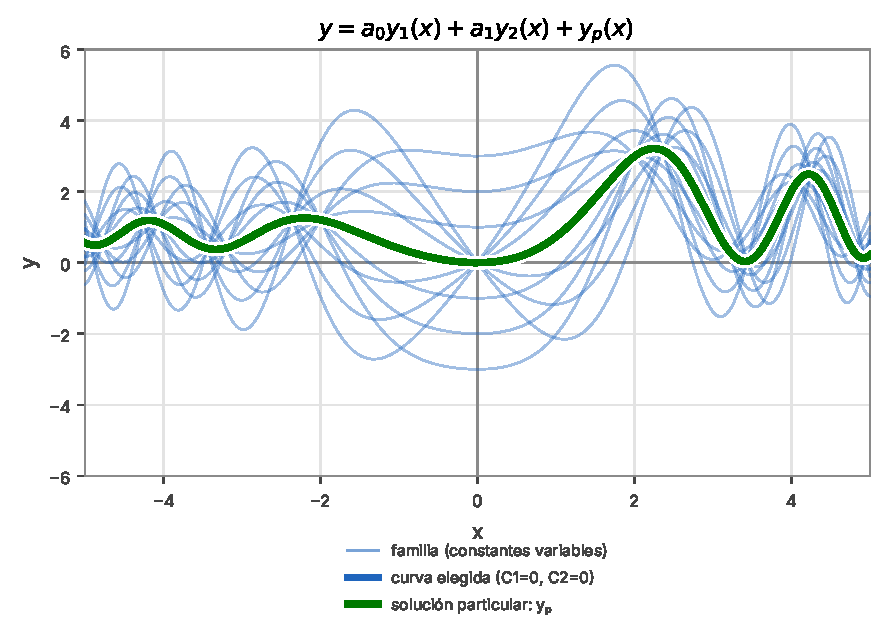
\includegraphics[width=0.8\linewidth]{h5-07.pdf}
\end{center}

\separador

\end{document}
